%%%%%%%%%%%%%%%%%%%%%%%%%%%%%%%%%%%%%%%%%%%%%%%%%%%%%%%%%%%%%%%%%%%%%%%
%%                                                                   %%
%%    Thesis and Term Paper Template                                 %%
%%    Created by Annemarie Friedrich                                 %%
%%                                                                   %%
%%    Original available from:                                       %%
%%    http://www.coli.uni-saarland.de/~afried/files/Term%20Paper.zip %%
%%                                                                   %%
%%    This header added by Dave Howcroft for the version at:         %%
%%    https://repos.lsv.uni-saarland.de/howcroft/texplates           %%
%%                                                                   %%
%%%%%%%%%%%%%%%%%%%%%%%%%%%%%%%%%%%%%%%%%%%%%%%%%%%%%%%%%%%%%%%%%%%%%%%

\documentclass[pdftex,12pt,a4paper]{article}

% Lorem ipsum filler text for the template
\usepackage{lipsum}

% For graphics
\usepackage[pdftex]{graphicx}
% Enables placing a figure at the position where it occurs in the text 
% by using [H]
\usepackage{here}

% For flexible tables
\usepackage{multirow}

% Set the encoding to UTF-8
\usepackage[utf8]{inputenc}

% Sophisticated citation.
% Check out: http://merkel.zoneo.net/Latex/natbib.php
\usepackage{natbib}

% Math symbols not defined in the usual package, e.g. arrows that are crossed.
\usepackage{amssymb}

% Arrows with text / superscript
\usepackage{amsmath}

% Different font - something like Arial
%\usepackage{mathptmx}

% Adjust margin of paper.
\usepackage{geometry}
\geometry{a4paper, top=25mm, left=25mm, right=25mm, bottom=25mm}

% Zeilenabstand 1.25 %
\linespread{1.2}

% Example Environments
\usepackage{amsthm}
\newtheoremstyle{style}   
  {0.5cm}              %Space above    
  {-0.8cm}              %Space below
  {}                      %Body font: original {\normalfont}    
  {}                      %Indent amount (empty = no indent,%\parindent = paraindent)    
  {\normalfont\bfseries}  %Thm head font original       
  {{\normalfont\bfseries \thmname{#1}\thmnumber{ #2}}}
\theoremstyle{style}
\newtheorem{example}{Example}[section]

% Formula Environments
\newtheorem{formula}{Formula}[section]

% Computational Linguistics trees etc.
\usepackage{xyling}

% Nicer captions
\usepackage{caption2}
\newcaptionstyle{mystyle}{%
  \normalcaptionparams
  \renewcommand\captionlabelfont{\bfseries}%
  \renewcommand\captionlabeldelim{.}%
  \onelinecaptionsfalse
  \usecaptionstyle{centerlast}}

\captionstyle{mystyle}

% Table of contents depth
\setcounter{tocdepth}{3}

% A horizontal rule for the title page
\newcommand{\HRule}{\rule{\linewidth}{0.5mm}}

% Paragraph and indent (as required by Prof. Dr. Pinkal)
\setlength{\parindent}{0pt}
\setlength{\parskip}{2ex plus 0.5ex minus 0.2ex}

\begin{document}

% Include the title page (modify title.tex!)
\begin{titlepage}
\begin{center}

% Upper part of the page. The '~' is needed because \\
% only works if a paragraph has started.

\includegraphics[width=0.25\textwidth]{images/uni-eule}~\\[1cm]

\textsc{\LARGE Saarland  University}\\[0.4cm]
\textsc{\Large Department of Language Science and Technology}\\[1.5cm]

\textsc{\Large Seminar:} \textbf{\Large Machine Learning for NLP}\\[0.5cm]

% Title
\HRule \\[1.0cm]

{ \huge \bfseries Exploring the limits of transfer learning with text-to-text transformer}\\[0.4cm]

\HRule \\[1.5cm]

% Author and supervisor
\begin{minipage}{0.4\textwidth}
\begin{flushleft} \large
\emph{Authors:}\\
Lakshmi \textsc{Rajendram Bashyam}\\
Matriculation: 2581455
\end{flushleft}
\end{minipage}
\begin{minipage}{0.4\textwidth}
\begin{flushright} \large
\emph{Supervisors:} \\
Dr. Dietrich  \textsc{Klakow}\\
\end{flushright}
\end{minipage}

\vfill

% Bottom of the page
{\large 31 October 2020}

\end{center}
\end{titlepage}


\thispagestyle{empty}
\begin{abstract}

Transfer learning has become widely popular learning technique in many applications specifically in a natural language processing setting. There can be many ways to transfer the knowledge from one setting to another. In this report, the popular technique of building pre-trained transfer models and its performance of downstream task is discussed in detail. \\
This type of transfer learning involves two steps, First is to train a machine learning model on a data rich task. Here, data rich task refers to the task for which data is easily available such as language modelling where the data can be simply scraped from the web pages which are abundantly available. This model called the pretrained model captures the low-level details of the task such as semantics or grammar of the language. Second step involves reusing this general-purpose knowledge gained by fine tuning the pretrained model on specific NLP tasks such as named entity recognition or sentiment classification task.\\ 
The paper “Exploring the limits of transfer learning with text-to-text transformer” extends this idea into a text-in, text out model that can be used across many NLP tasks. It also presents a detailed comparative study of different transfer learning techniques and incorporates the best performing methods to present the final model T5 along with the C4 dataset that was used to train it. Together it achieves state of the art performance at the time of its release on many NLP tasks. 


\end{abstract}
\newpage

% Table of contents
\thispagestyle{empty}
\tableofcontents

\newpage

% Start of content
\setcounter{page}{1}		% Seitenzähler auf 1 setzen %
%\pagestyle{fancy}				% fancy header style
\pagenumbering{arabic}
\newpage
\section{Base Architecture}

\subsection{Transformer}
The T5 model is largely based on the transformer architecture which was first introduced in “Attention is all you need” paper by Vaswani et al. The transformer architecture proposes to use attention mechanism as a replacement for then prevalent recurrent and convolution neural network to identify dependency between input and output tokens. 
\begin{figure}[H]
\centering
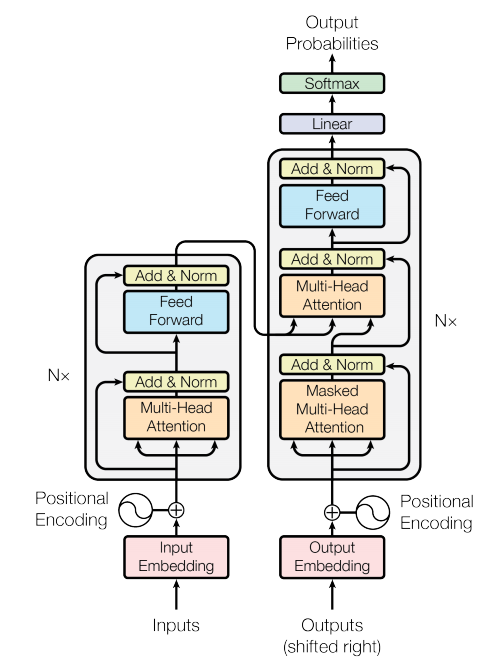
\includegraphics[width=0.7\textwidth]{images/transformer.png}
\caption{Transformer architecture}
\label{fig:transformer}
\end{figure}

The architecture consists of N stacked encoder followed by N stacked decoder layers. Each encoder layer consists of Multi head attention layer followed by feed forward layer, where the output from each of these layer passes through a layer normalisation. The decoder layer consists of the same components as encoder in addition to the masked multi head attention on the output tokens. Both the input and output tokens are vectorised by word2vec embedding and position of the tokens are encoded by a set of sine and cosine functions. The output from the decoder is then passed through a linear layer with SoftMax activation function to get the final results. 

\subsubsection{Attention}
In a traditional sequence model setting such as RNN or LSTM, there is a single context vector that captures the entire information of the input sentence. This context vector (or) hidden layer is used to generate output in the decoder layer. In case of sequence to sequence model, the context vector is passed through the decoder layer where it further encodes the decoder tokens at previous timesteps. This method works well for small sentences. \\
As the length of the sentence increases, the context vector is unable to encode all the information of the sentence in an efficient manner. \\
\begin{figure}[H]
\centering
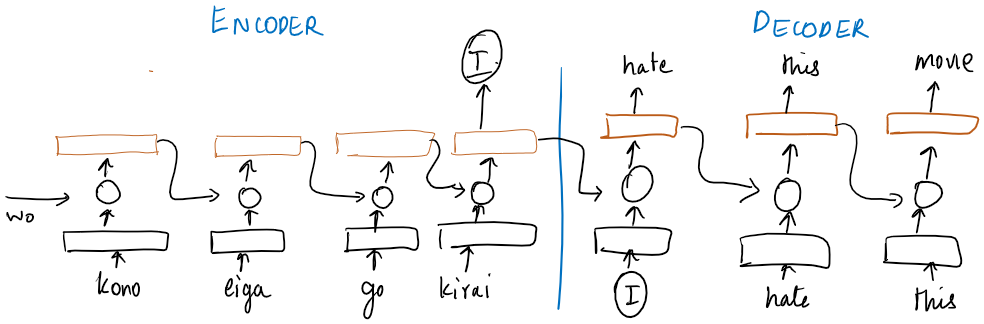
\includegraphics[width=0.9\textwidth]{images/rnn.png}
\caption{Encoder-decoder model}
\label{fig:rnn}
\end{figure}

Attention mechanism (Figure 3) weighs each term of sequence by focusing on relevant part of the sequence. The context vector of each token at decoder layer is calculated based on the contribution of each input token. Thus, the context vector encodes only relevant information at each time step. This enables it to process long sentences effectively and further preventing the vanishing gradient problem

\begin{figure}[H]
\centering
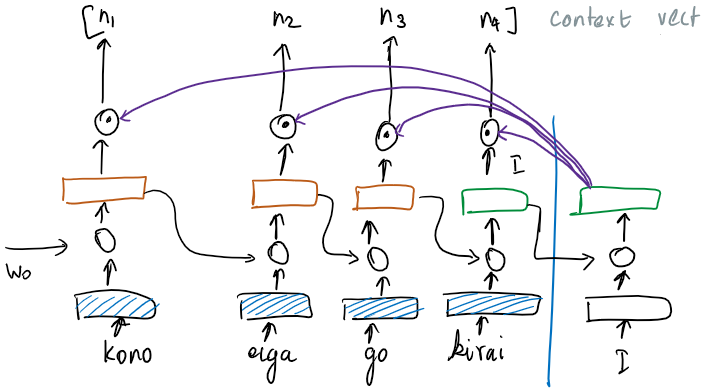
\includegraphics[width=0.7\textwidth]{images/attn.png}
\caption{Attention mechanism}
\label{fig:attn}
\end{figure} 
The Attention is computed from the formula \\
\(Attention(Q,K,V) = softmax((Q.K^{T})/ \sqrt{ d_{k} }).V\)
\\ Where K, V are the key value pair representing the encoder hidden state and Query Q represents the decoder hidden state

\subsubsection{Multi head attention}
Attention mechanism in both encoding and decoding layer is performed as Multi-head Attention. It helps to focus not just on different words in a sentence but also on different segments of the words. Each sentence is divided into h different blocks and attention is performed on each of these blocks. This step can be easily parallelized and the final representation of the sequence is the concatenation of result from each of these blocks.  \\
The output tokens are attended by Masked Multi head attention. It is essentially attention with Mask vector to ensure terms attend only to itself and previous time step terms. 

\begin{figure}[H]
\centering
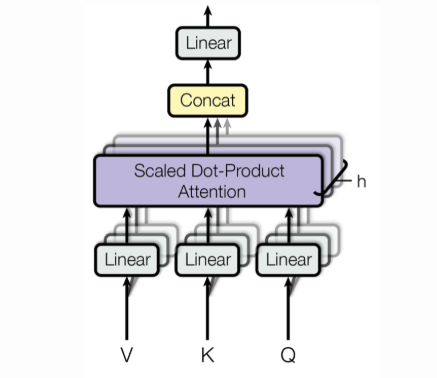
\includegraphics[width=0.4\textwidth]{images/mutlihead.png}
\caption{Multi head attention}
\label{fig:multihead}
\end{figure} 

\subsubsection{Self attention}
The Multi head attention at encoding layer and Masked multi head attention at decoder layer performs Self-attention. Self-attention is similar to attention mechanism where both Query and Key, Value pair are same. Thus, it can be seen as a representation of the sequence by relating different positions of a single sequence.
\begin{figure}[H]
\centering
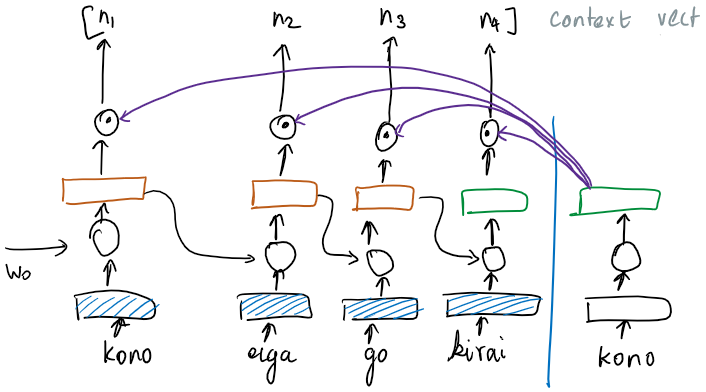
\includegraphics[width=0.7\textwidth]{images/selfattn.png}
\caption{Self Attention}
\label{fig:selfattn}
\end{figure} 

\subsection{Text-to-Text Transfer Transformer}
The Text to text transfer transformer, hence the name T5, model is a Transformer that takes text as an input and returns text as output. The input text consists of prefix that represents task objective such as sentence similarity or sentiment classification followed by the original text input. The output of the NLP tasks which maybe a classification output, number or part of the input text are also modelled in text format. As an example, In case of machine translation task, \\
The input text is “translate Japanese to English: Kono eiga ga kirai”\\
The output text is “I hate this movie”

\subsubsection{Architecture}
The T5 model consists of same transformer model that was discussed earlier except for following changes,
\begin{enumerate}
\item At the layer normalisation, the bias is removed and the it is placed outside the residual skip connection
\item The position of the tokens in the sequence are encoded based on the relative position from one another. 
\item Word piece embedding that considers combination of word vectors and character encoding from a fixed vocabulary instead of word2vec. 
\end{enumerate}
It consists of 12 layers of encoder and decoder layers followed by a feed forward layer with output layer of 3072 dimensionality and dropout layer with dropout probability of 0.1, 12 attention heads. Together the baseline model has about 220 million parameters. This is similar to the parameter setting of the BERT-base model.
\subsection{Colossal clean crawled corpus}
Large amount of data is required for training the T5 model. Usually the pre-training task is unsupervised in nature, such as language modelling or de-noising. In such a case, data crawled from web pages can be used as the pre-training dataset. 
The dataset is obtained by preprocessing the publicly available common crawl dataset. The preprocessing involves removing punctuation, offensive sentence, duplicate sentences and sentences containing code. Additionally, a language filtering is performed on top of it to retain only English language texts. The resulting dataset is colossal clean crawled corpus, named C4 dataset that is used for pre-training the T5 model. 






\newpage
\section{Study of Transfer learning methods}
\subsection{Downstream Task}
The performance of pre-trained T5 model is verified on following NLP benchmarks. \textbf{In this report, the findings are reported only on GLUE tasks considering space constraints. For full complete set of results, please refer the original paper. }
\begin{enumerate}
    \item GLUE and Super GLUE task: It comprises of diverse set of tasks to test the natural language understanding abilities including 
    \begin{enumerate}
        \item Sentence acceptability 
        \item Sentence analysis
        \item Sentence similarity
        \item Natural language inference
        \item Co-reference resolution
        \item sentence completion
        \item Word sense disambiguation
        \item Question answering
    \end{enumerate}
    \item Text summarization on CNN/Daily Mail
    \item Question answering on SQuAD dataset
    \item English to German, English to French, English to Romanian Machine translation 
\end{enumerate}

\subsection{Architecture}
The main differences in the architecture design in transfer learning setting arise from the type of masking used in the model. Masking is used to impose constraints on which tokens in the sequence the input token can attend to. \\
In the case of encoder-decoder architecture (Left in figure), The encoder block uses fully connected mask wherein each token in the input is a weighted sum of all the tokens in the sequence and the decoder layer uses causal masking, where each input in the sequence can only attend to itself and previous tokens in the sequence. Similarly, a language model (middle in figure) which predicts the next word in a sequence also uses causal masking, whereas models such as BERT uses fully connected masking.\\
It is also possible to extend language models for other NLP task by concatenating the inputs and targets. For example, in case of machine translation from Japanese to English, the input to a language model would be “translate Japanese to English: Kono eiga ga kirai target: I hate this movie”. But using causal masking in this setting might restrict the model to use only a limited input token. To counter this drawback, Prefix LM masking (right in figure) can be used in language models. Prefix ML has a fully connected masking for fixed input tokens and a causal masking for the rest of the tokens. This allows the Language model to use all of the input tokens to predict the output word by word language modelling style. \\
It is also possible to compare architectural variants in terms of number of parameters P and amount of computation M required to process a given input sequence. 
On comparison the encoder-decoder model with de-noising objective having 2P parameters and M computational cost was found to perform better than all other variants. \\

\begin{figure}[H]
\centering
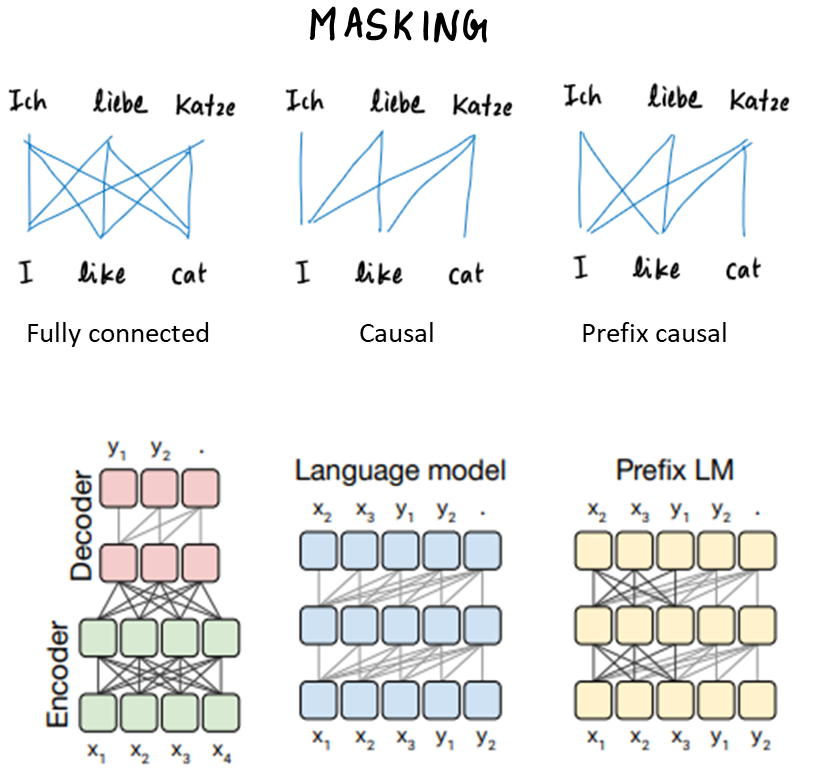
\includegraphics[width=0.7\textwidth]{images/masking.png}
\caption{Masking}
\label{fig:masking}
\end{figure} 

\subsection{Pre-training Objective}
In addition to the language modelling objective from the previous section, there are many other widely adopted strategies to train an unsupervised transfer learning model. \\
One of the most commonly used method is the de-noising objective where the some of the tokens in the input text is replaced by <M> tag. The objective of the model is to reconstruct the input sequence. It has many variants in itself. 

\begin{enumerate}
   


  \item The BERT style de-noising where the certain tokens are replaced by the <M> tag and some of them are replaced by random words \\ Input: Thank you <M> <M> me to your party apple week. \\Output: Thank you for inviting me to your party last week 
  \item MASS style is similar to BERT without the random word replacement \\ Input: Thank you <M> <M> me to your party last week.  \\ Output: Thank you for inviting me to your party last week  
  \item Deshuffling where the objective is to identify the correct order of the shuffled input tokens  \\ Input: party me for your to . last fun you inviting week Thank  \\  Output: Thank you for inviting me to your party last week.  
  \item Replacing spans of tokens instead of single token \\ Input: Thank you me to your party week   \\  Output: Thank you for inviting me to your party last week.
\end{enumerate}
Comparing a more detailed approach to corruption strategy, it is possible to adjust the corruption token length and corruption rate, in other words the number of tokens corrupted with respect to length of input sequence to monitor its impact on the performance measure. \\
Out of all the variants, BERT style pre-training objective that replaces 15 percent spans of length 3 achieves a better performance. 
\begin{figure}[H]
\centering
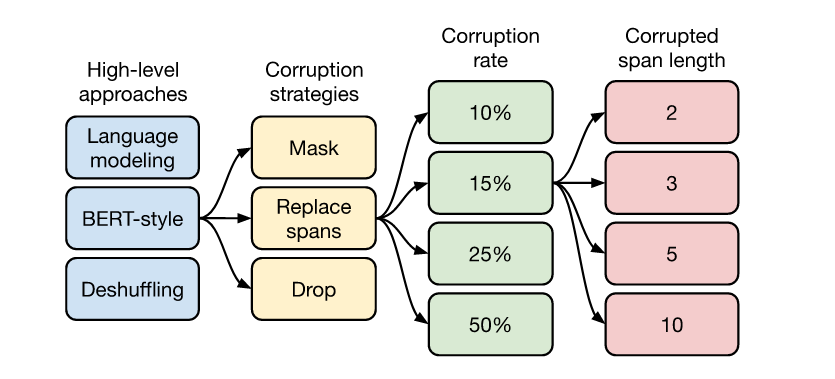
\includegraphics[width=0.7\textwidth]{images/preobj.png}
\caption{Pre-training objective}
\label{fig:preobj}
\end{figure} 

\subsection{Pre-training dataset}
Pre-training dataset is a very essential part of the transfer learning model. The quality and the type of the dataset might have a considerable effect on the performance of downstream and hence it is necessary to compare the different types of commonly used pre-training datasets. \\
Along with the C4 dataset previously discussed, the comparison was made on non-pre-processed C4 dataset, data extracted from Wikipedia, news dataset, data from content aggregation sites such as reddit, Wikipedia and book corpus. \\
The findings are presented in figure (right) below. It can be observed that Real news and Web text gives a better performance on glue tasks than the C4 dataset. Similarly, Wikipedia + TBC produces good performance on Super Glue task. The reason was identified as relatively high performance on MultiRC task of GLUE and Super GLUE which comes from a similar domain as the former dataset.  Thus, it can be argued that pre-training on in-domain unlabelled data can improve performance on downstream tasks. \\
In addition to dataset type, it is also beneficial to study the effect of repeating examples on performance of pre-training model. By repeating the data set 64, 256, 1,024, and 4,096 times during pre-training process, it is observed from the figure (left) below that the performance degrades as more and more examples are repeated during the training phase. 

\begin{figure}[H]
\centering
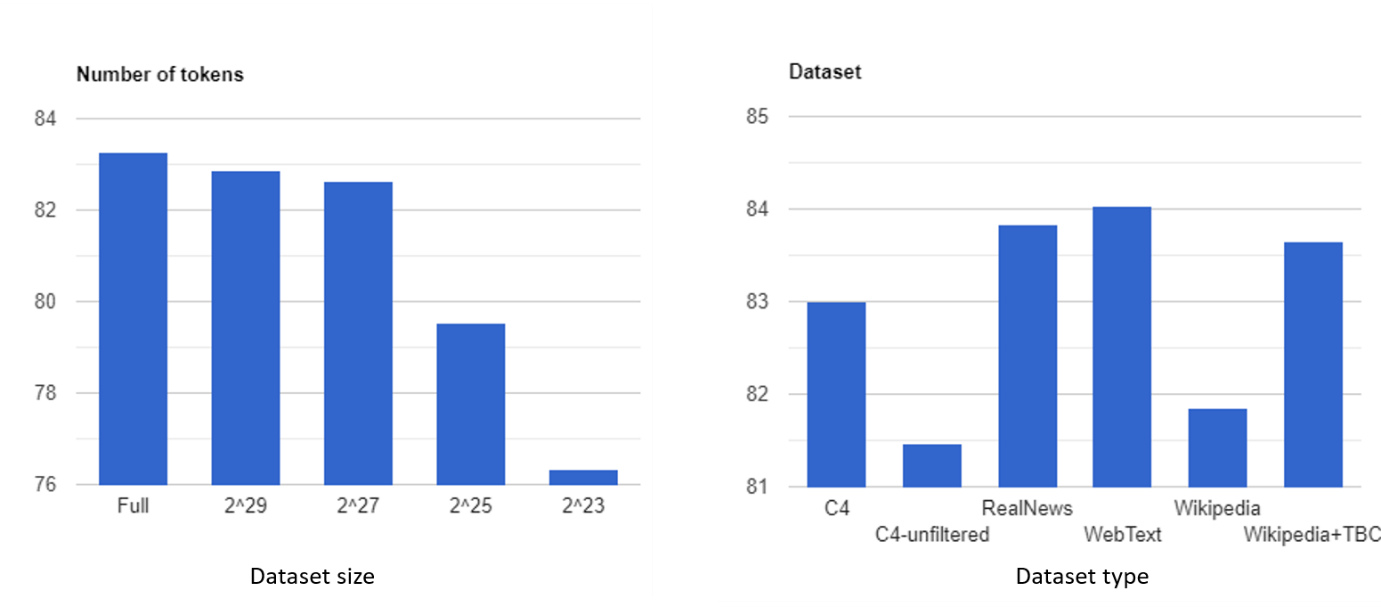
\includegraphics[width=0.7\textwidth]{images/predataset.png}
\caption{Pre-training Dataset}
\label{fig:predataset}
\end{figure}

\subsection{Downstream fine tuning}
Common approach to fine tuning on downstream is to fine tune only the last layers of the pre-trained model. This approach is usually seen in popular models such as BERT, XLNET. But in case of an encoder decoder architecture like T5 model, it is ideal to fine tune on all of the parameters of the model. But this computationally heavy and time consuming. \\
One of the alternate approaches considered here is the Adaptive layers approach. In this method, a dense ReLu block is added on top of each feedforward layer in the T5 model. This ReLu block has the same dimensionality d as the feed-forward layer and the parameters of the ReLu block alone is fine-tuned while training the model in the downstream task. It is observed that this method works well on low resource tasks such as SQUAD. \\
Another method is the Gradual unfreezing, where the parameters of the layers are fine tuned in a bottom up style. In other words, at first iteration the parameters of final layer are fine-tuned, in the second iteration last two layers are fine tuned and so on. Even though the performance of this method comparatively lower than fine tuning all of the parameters, it takes far less time than the latter approach. \\


\begin{figure}[H]
\centering
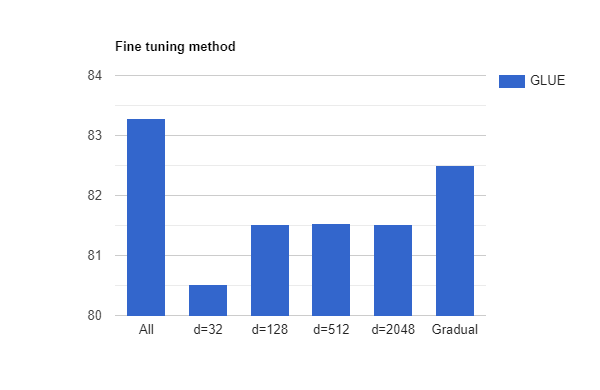
\includegraphics[width=0.7\textwidth]{images/finetune.png}
\caption{Downstream fine tuning}
\label{fig:finetune}
\end{figure}

\subsection{Multi task learning}
In order to incorporate the ability to perform multiple tasks simultaneously into the model, it is sufficient to mix training data from all of theses tasks since the T5 model is already defined as a text-to-text model. \\
Among the different methods, examples proportional method mixes data at the rate of  \\
\(r_{m} = min( e_{m},K)/ \sum min( e_{n},K)  \)
\\ Temperature scaled method is similar to the examples proportional method where the value of rm is raised to a power of T. The value of T limits how much the larger dataset is mixed. 
From the figure below it can be identified that for a specific value of K, the examples proportional methods works well and the temperature scaled method achieves even higher performance for a T value of 2. 

\begin{figure}[H]
\centering
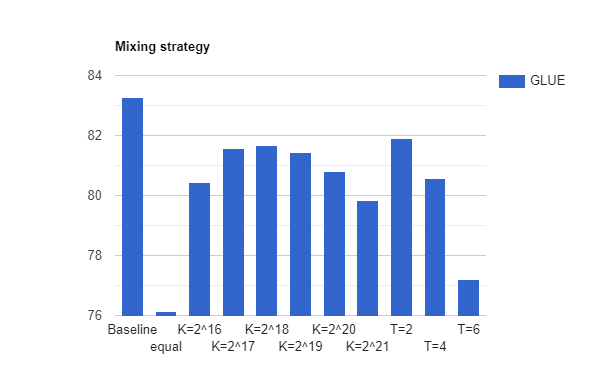
\includegraphics[width=0.9\textwidth]{images/multitask.png}
\caption{Multi task learning}
\label{fig:multitask}
\end{figure}

\subsection{Scaling}
It is very common in the transfer learning domain to improve the performance of the model significantly simply by scaling up the model in terms of model size S, training steps T or ensemble model E. 
With the assumption of 4 times more computational power, different scaling strategies are compared and it can be concluded that increasing both the model size and number of steps simultaneously achieves a significant increase in performance compared to other methods. 
The T5 large model is configured similar to BERT large model and consists of 4096 feedforward dimension, 16 attention head, 16/32 layers encoder-decoder block. The T5 3B model 16384 – feedforward layer dimension, 32 attention head and T5 11B model has 65538 – feedforward layer dimension, 128 attention head.

\newpage
\section{Summary}
The final T5 architecture was modelled as a Text-to-text architecture that provides a unified approach. Along with the common crawl C4 dataset it achieves state of the art performance on many of the NLP tasks. A very detailed comparative study was performed which compared different types of architecture such as BERT style, Language modelling and encoder-decoder model along with their pre-training objectives where the denoising method with spans was found to produce the best results. On comparing different dataset full C4 dataset without any repetition was selected as the best method. While comparing different mixing methods, no clear best method was distinguishable but it gave a comparable performance. For fine tuning the pre-trainined model obtained above on downstream task, it is beneficial to look at methods such as gradual freezing which significantly reduces the time to train. Finally the scaling strategy significantly increase the performance from the baseline architecture providing state of the art performance. \\\\
Even though it has achieved a high accuracy, the architecture of the T5 model remains relatively same to the transformer architecture. Since we use a English language filter on the dataset it cannot be extended easily to other languages. It also might be required to find a balance between computational cost and performance to increase adoption in practical setting. 


% REFERENCES
\newpage

\bibliographystyle{apalike}

\bibliography{references}
\cite{raffel2020exploring}
\cite{NIPS2017_7181}
\cite{devlin-etal-2019-bert}
\cite{JayAlammar.2018}
\cite{Google_AI_blog.2020}
\end{document}